%\documentclass{acm_proc_article-sp}
\documentclass{sig-alternate}
\usepackage{amsmath}
\usepackage{amssymb}
\usepackage{listings}
\usepackage{courier}
\usepackage{multirow}

% Include PDF graphics, configure our images directory, and specify image types.
\usepackage{graphicx}
\usepackage{epsfig}
\graphicspath{{./images/}}
\DeclareGraphicsExtensions{.pdf,.jpeg,.png,.jpg}

% Style listings
\lstset{%rulesepcolor=\color{Gray},
        frame=single,                        	% Shadow box frame around code
        basicstyle=\scriptsize\ttfamily,        % Use small true type font
        showstringspaces=false,                 % Don't put marks in string spaces
        morecomment=[l][\color{Blue}]{...},     % Line continuation (...) like blue comment
}

\begin{document}

\title{Toward Quantitative Emulation of Cloud Robotic Systems}

\numberofauthors{1}

\author{
\alignauthor
Christopher C. Lamb, Rafael Figueroa, Rafael Fierro\\
       \affaddr{University of New Mexico}\\
       \affaddr{Department of Electrical and Computer Engineering}\\
       \affaddr{Albuquerque, NM 87131-0001}\\
       \email{\{cclamb, rafa, rfierro\}@unm.edu}
}

\conferenceinfo{ICCPS '14,} {April 14-17, 2014, Berlin, Germany.} 
\CopyrightYear{2014} 
\crdata{978-1-4503-1005-5/11/10} 
\clubpenalty=10000 
\widowpenalty=10000

\maketitle

\begin{abstract}
Networks of collaborating autonomous cyber-physical systems are just beginning to be able to take advantage of cloud computing.  As the advantages of using cloud computing become more obvious and validated in other fields, cloud computing will inevitably begin to migrate into autonomous system development.  Our goal overall is to begin to provide quantitative guidance around how system developers can take advantage of cloud computing within their systems.  In order to do this, we have embarked on two specific research thrusts; the first, building a cloud computing framework specifically tailored to the unique needs of autonomous systems, and the second, developing the appropriate simulation, emulation, and other tools needed to facilitate autonomous system cloud development.  Our first step, outlined within this paper, is to develop an initial taxonomy of the types of distributed system architectures system developers will likely use, to notionally describe where and when they should be used, and how they could be developed and integrated.
\end{abstract}

\category{D.2.11}{Software}{Software Architectures}[Domain-specific Architectures]
\terms{Design, Performance, Robotics}
\keywords{Robotics, Cloud}

\section{Introduction}
In the last two years, the robotics and autonomous systems community has begun looking closely at cloud computing to determine its efficacy in helping shoulder the computational load of systems.  Overall, the consensus is that cloud computing is positioned to make as large as an impact in robotics over the next few years as it has in general Information Technology in the last.  Projects that have begun to explore distributed knowledge management have demonstrated promising results~\cite{TeKlPaBe:11, TePeLaBe:12, WaBeCiDa:11}, and have spawned other similar approaches in related domains.

We believe this approach to using cloud computing to help shoulder the computational burden for autonomous systems is not only promising, but here to stay, and also fraught with unique challenges.  First, the economic benefits seem undeniable.  Just as the cost and flexibility of cloud systems provided by commercial service providers like Amazon and Rackspace have encouraged an exodus of processing power from the company data center to the cloud, similar flexibility and cost savings will exist for robotics engineers.  Today, in order to provision a network of robots, researchers need to acquire and administer laboratory computers, networks, and robotic systems prior to making any progress.  Furthermore, these resources are centralized within a single laboratory and are usually inaccessible remotely.  This leads to the very problem cloud computing set out to solve; an high capital-intensive barrier to entry and  inconvenient resource centralization.  Incorporating cloud computing into typical experimental environments makes processing power and storage more accessible than ever before, promising to bring new engineers into robotics as the Arudino brought programmers into the world of micro-controllers.  

Not only can cloud computing lower barriers to entry, it can also more effectively provide processing power to networked autonomous systems.  Instead of requiring local data storage and processing power, or planning systems that while remote are still centralized on a single workstation in a laboratory, the ability to take advantage of the virtually unlimited computational resources of cloud computing allows robots to run just about anywhere, distributing computation allows for resoure intensive applications to be offloaded from robots to inexpensive cloud systems.

While the argument in favor of cloud computing for robotic systems mirrors that used with respect to traditional server-based computing, there are some distinct differences between the computation, storage, and communication needed by autonomous systems as opposed to simple servers or workstations.  For example, communication latencies have a much larger impact on autonomous systems than non-mobile systems.  An actuator managing a floodgate and controlled by cloud-integrated micro-controller afford to wait for direction from an external service under flood conditions.  Likewise, a cloud-enabled grasping arm needs to be able to quickly acquire grasping information from external sources whenever confronting a new object.  

In order to effectively build these kinds of systems, we must first understand what kinds of systems we could build, under what circumstances, and why.  

\section{Cyber-physical Clouds}
Highlight the problem we are starting to address.

\subsection{A Taxonomy of Architectures}
Outline an initial taxonomy.

\subsection{Initial Analysis of Taxonomy}
Notionally analyze the taxonomy.

\subsection{Future Work}
Where to next.

\section{Related Work}
Cover previous work in area, especially motivating work.

\section{Summary and Conclusions}

%\begin{figure}[!t]
%\centering
%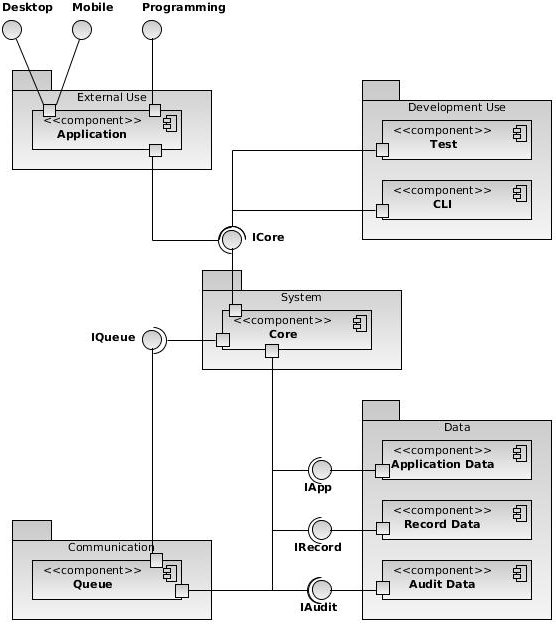
\includegraphics[width=3in]{HisbSystemArch}
%\caption{System Architecture Runtime Component View}
%\label{fig:RuntimeView}
%\end{figure}

\bibliographystyle{abbrv}
\bibliography{bib/cps.bib}

\end{document}


